
%(BEGIN_QUESTION)
% Copyright 2012, Tony R. Kuphaldt, released under the Creative Commons Attribution License (v 1.0)
% This means you may do almost anything with this work of mine, so long as you give me proper credit

Kombiner ligningene $U = IR$, $I_{total} = I_1 + I_2$ og $U_{total} = U_1 = U_2$ for denne parallellmotstandskretsen for å løse for $I_{total}$ som en funksjon av $U_{total}$, $R_1$ og $R_2$. Med andre ord: skriv en ny ligning med bare $I_{total}$ på den ene siden av likhetstegnet, og uten andre variabler enn $U_{total}$, $R_1$ og $R_2$ på den andre siden:

$$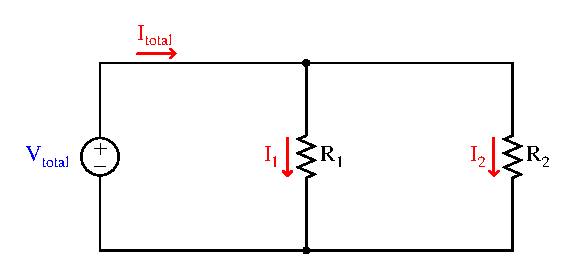
\includegraphics[width=15.5cm]{i01330x01.eps}$$

$$I_{total} = f(U_{total}, R_1, R_2)$$

\underbar{file i01330}
%(END_QUESTION)





%(BEGIN_ANSWER)

$$I_{total} = {U_{total} \over R_1} + {U_{total} \over R_2}$$

Slik kommer vi fram til dette svaret:

\begin{itemize}
\item{} Først identifiserer vi variabelen vi skal løse for. I dette tilfellet er det $I_{total}$.
\vskip 10pt
\item{} Deretter finner vi hvilken av de oppgitte ligningene som inneholder denne variabelen. Her er det $I_{total} = I_1 + I_2$.
\vskip 10pt
\item{} Så ser vi etter måter å erstatte $I_1$ og $I_2$ i den første ligningen med uttrykk som inneholder $U$- og $R$-variablene.
\vskip 10pt
\item{} Vi vet fra Ohms lov at $U = IR$. Derfor er $U_1 = I_1 R_1$ og $U_2 = I_2 R_2$.
\vskip 10pt
\item{} Vi setter så inn $U_1 \over R_1$ for $I_1$, og $U_2 \over R_2$ for $I_2$. Resultatet blir $I_{total} = {U_1 \over R_1} + {U_2 \over R_2}$.
\vskip 10pt
\item{} Ved å bruke likheten $U_{total} = U_1 = U_2$ for parallellkretser, erstatter vi nå $U_1$ og $U_2$ med $U_{total}$ og får $I_{total} = {U_{total} \over R_1} + {U_{total} \over R_2}$.
\end{itemize}


%(END_ANSWER)





%(BEGIN_NOTES)


%INDEX% Mathematics review: basic principles of algebra
%INDEX% Mathematics review: manipulating and combining equations to form a new equation

%(END_NOTES)
